\problemname{Security Check}

As Exalted Foreman of the Darven miners' union it is your job and privilege to tell the other dwarves when they can stop working.
You do this by announcing the Dwarvish equivalent of “The shift is over!” in a loud voice.
This is heard by everybody in the same hall you're in, but by nobody else.
To inform the remaining miners in the vast tunnel system, you must walk through the mines and repeat the announcement in each of the other halls.
Since walking through tunnels takes time,
you will invariably be late with your announcement in the other halls.
The later you are, the more grumpy will the dwarves in that hall be, which incurs a penatly to your social status, authority, and popularity.

You want to plan your route so as to incur the smallest total penalty. 

\medskip
The Dwarven mines consist of $n$ halls and $n-1$ tunnels.
The entire system is connected, so it is possible to get from any hall to any of the others.
It takes one unit of time to traverse a tunnel.
Announcing the end of shift and traversing a hall takes no time.
In each hall, announcing the end of shift $t$~time units late incurs a penalty of~$t$.
You may not announce the end of shift early in any of the halls.
You can start in any of the halls.

\subsection*{Example}

In sample input~$1$, the mines look like this:


\includegraphics[width=.15\textwidth]{img/sample-1.pdf}

If you start in hall~$2$ and visit the rest of the mines in the order $2$, $1$, $2$, $3$, you can announce the end of shift at time~$0$ (in hall $2$), time~$1$ (in hall $1$), and time~$3$ (in hall $3$).
The total penalty for this route is $0+1+3=4$.
If instead you start in hall~$1$ and visit the mines as $1$, $2$, $3$, the total penaly is $0+1+2=3$, which is better.

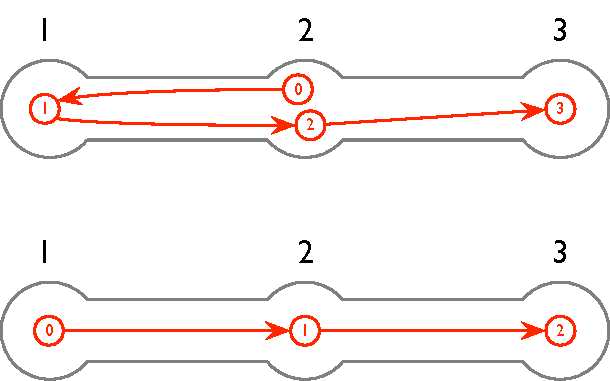
\includegraphics[width=.35\textwidth]{img/sample-1-ans.pdf}

\subsection*{Input}

The first line of input consists of the integer $n$, the number of halls.
We assume that $1\leq n\leq 100\,000$ and that the halls are numbered $1$, $\ldots$, $n$.
The next $n-1$ lines each contain two space-separated integers $u$ and $v$ with $1\leq u < v \leq n$, meaning that there is a tunnel between hall~$u$ and hall~$v$.

\subsection*{Output}

Print a single integer: the minimum possible penalty.

\subsection*{Constraints}

Your solution will be tested on a set of test groups, each worth a number of points.
Each test group contains a set of test cases.
To get the points for a test group you need to solve all test cases in the test group.
Your final score will be the maximum score of a single submission.

\medskip
\begin{tabular}{lll}
Group & Points & Constraints \\\hline
1 & 18 & no hall is incident to more than two tunnels\\
2 & 19 & at most one hall is incident to more than two tunnels\\
3 & 20 & $n\leq 10$\\
4 & 21 & $n\leq 1\,000$\\
5 & 22 & \emph{no additional constraints}
\end{tabular}
